
\section{Ocean Radar Backscatter (ORB)}
\label{sec:orb}
The ORB product is relatively straightforward to derived from the NRB product. Therefore, most of the critical processing steps have been addressed during NRB product generation. In addition to the NRB input, the generate of the ORB products requires ERA5 wind data and geophysical model functions (GMF). The ORB product includes multiple layers of $\sigma_{0}$ values, each corresponding to a specific processing stage: a full-resolution outlier mask in $\sigma_{0}$ convention, spatially averaged noise-equivalent $\sigma_{0}$, denoised $\sigma_{0}$, denoised and outlier-removed $\sigma_{0}$, and angle-of-incidence compensated $\sigma_{0}$.
\subsection{Evaluation criteria}
\label{sec:orb_criteria}
The main layer of the ORB products are the spatially-averaged, denoised, and outlier-removed $\sigma_{0}$, and the angle-of-incidence-compensated $\sigma_{0}$. The quality of the former is assessed through statistical analysis of the product itself, whereas the latter is evaluated through inter-comparison of results derived from Sentinel-1 C-band and SAOCOM L-band observations.

Using an example from SAOCOM observations, the performance of the outlier removal processing is summarized in Table \ref{tab:stats_sigma0}, which presents the statistics of the raw $\sigma_{0}$, identified outliers $\sigma_{0}$, and the resulting outlier-free $\sigma_{0}$.
\begin{longtblr}[
	label = tab:stats_sigma0,
	entry = none,
	caption = {Statistics of different layer of $\sigma_{0}$},
	]{
		width = \linewidth,
		colspec = {Q[l,20]Q[c,20]Q[c,20]Q[c,20]},
		hlines,
		hline{1-Z} = {-}{0.05em},
	}
	\textbf{Statistics}   & \textbf{$\sigma_{0,\mathrm{raw}}$}   & \textbf{$\sigma_{0,\mathrm{outlier}}$} & \textbf{$\sigma_{0,\mathrm{L}}$} \\
	Mean & 0.06 & 0.67 & 0.06 \\
    Median & 0.04 & 0.33 & 0.04 \\
    Standard deviation & 0.50 & 4.34 & 0.23 \\
\end{longtblr}
According to the statistics, the mean and median of the $\sigma_{0}$ values are preserved after the outlier removal, while the standard deviation is reduced by approximately $50\%$.

A comparison of Sentinel-1 and SAOCOM results is illustrated in Figure \ref{fig:orb_sentinel_saocom}.
\begin{figure}[ht!]
\centering
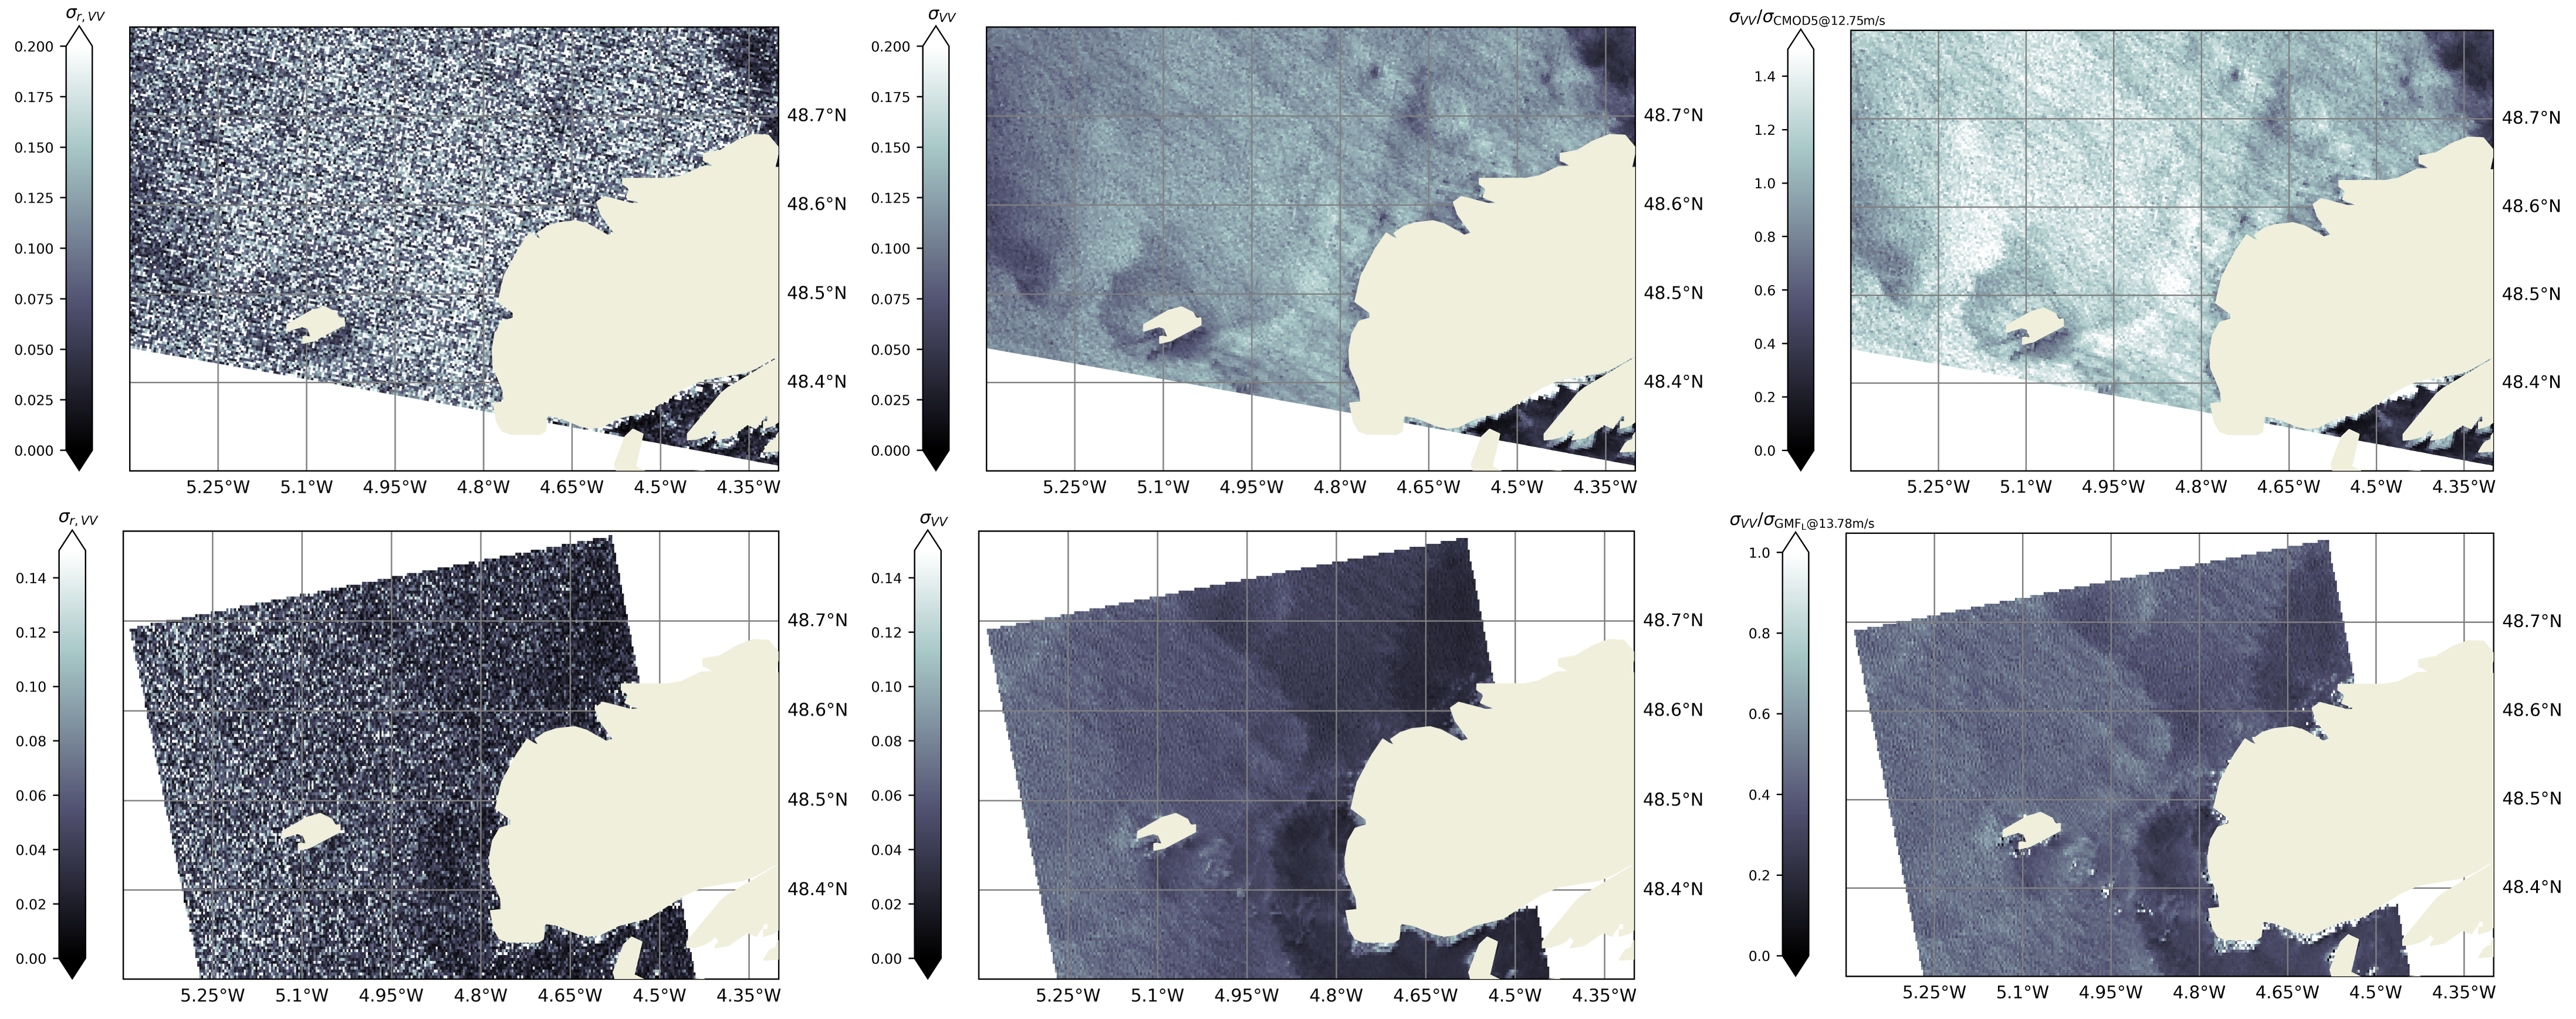
\includegraphics[width=0.9\textwidth]{Figures/oceans/D5_sentinel_saocom.png}
\caption{ORB products comparison between Sentinel-1 (upper panel) and SAOCOM (lower panel).From left to right are raw $\sigma_{0}$, denoised and outlier-free $\sigma_0$, and the angle of incidence compensated $\sigma_{0}$.}
\label{fig:orb_sentinel_saocom}
\end{figure}
Both observations were acquired on the same date, 2023-11-03, with the SAOCOM acquisition at 06:00:43 occurring approximately half an hour earlier than the Sentinel-1 acquisition at 06:32:31. Despite differences in acquisition mode, geometry and frequency, and the highly dynamic nature of the ocean, the roughness values in the ORB products exhibit comparable magnitudes.
\subsection{Theoretical models}
\label{sec:orb_models}
The processing of ORB products involves two essential steps: bright target removal and angle-of-incidence compensation, both of which incorporate theoretical models.
\subsubsection{Bright target removal}
To identify the bright target statistically, the sigma0 is low-pass filtered with a Gaussian window
\begin{equation}
    I^{\mathrm{LPF}}(x,y) = I(x,y)*h_{\mathrm{LP}}(x,y),
\end{equation}
with
\begin{equation}
    h_{\mathrm{LP}}(x,y) = \frac{1}{\sigma_x\sigma_y\sqrt{2\pi}}e^{-\frac{x_{i}^{2}}{2\sigma_{x}^{2}}-\frac{y_{i}^{2}}{2\sigma_{y}^{2}}},
\end{equation}
the impulse reponse of the Gaussian filter, where $\sigma_{x,y}$ are the filter widths, which can be in the order of km. We then compute the intensity contrast as
\begin{equation}
    K(x,y) = \frac{I(x,y) - I^{\mathrm{LPF}}(x,y)}{I^{\mathrm{LPF}}(x,y)}.
\end{equation}
Pixels for which the intensity contrast exceeds a given threshold,
\begin{equation}
    K(x,y) >K_{\mathrm{thres}}
\end{equation}
are considered outliers. Consequently, a mask is generated according to 
\begin{equation}
    M(x,y) = \begin{cases}
    1, & \text{if } K(x,y) < K_{\mathrm{thres}} \\
    0,  & \text{if } K(x,y) > K_{\mathrm{thres}}
    \end{cases}.
\end{equation}

To define the contrast threshold, we assume the intensity distribution of a single-look pixel is exponential, then the mean and standard deviation of the intensity are equal to $\frac{1}{\lambda}$. The summation of multiple independent exponential distributions changes the statistics. According to error propagation law, the mean and the standard deviation is scaled with the number of independent samples, in this case, the equivalent number of looks (ENL). The mean and the standard deviation are
\begin{equation}
    \mu = \frac{\mathrm{ENL}}{\lambda}, \sigma = \frac{\sqrt{\mathrm{ENL}}}{\lambda}.
\end{equation}
Therefore, the standard deviation can be written as a scaled mean
\begin{equation}
    \sigma = \frac{\mu}{\sqrt{\mathrm{ENL}}}.
\end{equation}
After the outlier removal, the energy loss due to the mask is restored. This is done by dividing the masked $\sigma_0$ by the low-pass filtered mask. Then, the noise-floor is subtracted. 
\begin{equation}
    \sigma_{0,\mathrm{L}} = \frac{(I(x,y)\cdot M(x,y))*h_{\mathrm{LP}}(x,y)}{M(x,y)*h_{\mathrm{LP}}(x,y)}-\mathrm{NESZ}.
\end{equation}
After these steps, the downsample is performed by using the resolution of the input data and the user desired resolution as input parameters.
\subsubsection{Angle of incidence compensation}
This step involves feeding a GMF with ERA5 wind products and the SAR imaging geometry. The angle-of-incidence compensation is then performed by scaling the downsampled product using the ratio $\sigma_{0,\mathrm{L}} / \sigma_{0,\mathrm{mod}}$, where $\sigma_{0,\mathrm{L}}$ is the locally observed backscatter and $\sigma_{0,\mathrm{mod}}$ is the GMF-predicted backscatter. The GMF for NRCS over ocean is generally expressed as:
\begin{equation}
    \sigma_{0,\mathrm{mod}}  = A_0(w,\theta)(1 + A_1(w,\theta)\cos{\varphi}+A_2(w,\theta)\cos{2\varphi}),
\end{equation}
where $\varphi$ is the relative wind direction with respect to the radar, $A_n(w,\theta)(n=0,1,2)$ is a function of wind speed $w$ and the incident angle $\theta$. For modeling NRCS from co-polarized L-band acquisitions, the definition of each $A$ function follows \cite{isoguchi_l-band_2009}, while for C-band, the forward CMOD5.N model is used.
\subsection{Computational performance}
\label{sec:orb_computation}
The computational load of generating the ORB product is comparable to that of the NRB product, although the ORB product includes more layers. The most computationally expensive step is the 2D Gaussian blurring, which is applied three times during the outlier removal process. For a single image, the total processing time of generating ORB from NRB is approximately $12.7$ seconds.
\subsection{Criticalities and weakness}
\label{sec:orb_criticalities}
Any quality assessment of the ORB product depends on the quality of the input NRB data, wind data, and geophysical model function (GMF), rather than the ORB algorithm itself. It remains unclear whether a local or global mean wind reference is more suitable for roughness computation, as each approach has its own advantages and limitations. At present, we use the local mean wind as a reference, as it provides better compensation for the angle of incidence dependence. 